\section{System Overview}


    \begin{itemize}
        \item \textbf{Frontend:}
        \item \textbf{Backend API:}
        \item \textbf{Reels Service:}
        \item \textbf{Database:}
    \end{itemize}

    \begin{figure}[htbp]
        \centering
        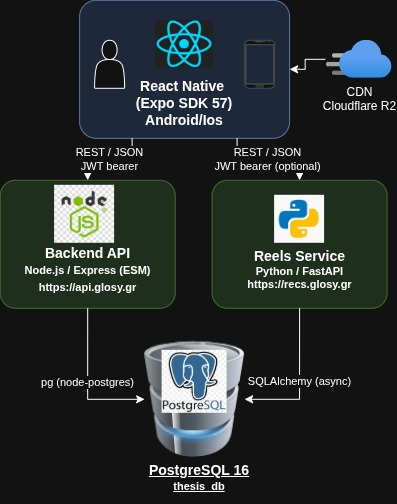
\includegraphics[width=0.85\textwidth]{figures/architecture.pdf}
        \caption{High-level system architecture: the mobile frontend communicates with the Backend API (\texttt{api.glosy.gr}) and the Reels Service (\texttt{recs.glosy.gr}) over authenticated REST endpoints; both services share a single PostgreSQL instance.}
        \label{fig:architecture}
    \end{figure}


\section{Technology Stack}
\label{sec:tech_stack}
    \subsection{Frontend --- React Native / Expo}
    \label{subsec:frontend_stack}

    \subsection{Backend API --- Node.js / Express}
    \label{subsec:backend_stack}

    \subsection{Reels Service --- Python / FastAPI}
    \label{subsec:reels_stack}

    \subsection{Database --- PostgreSQL}
    \label{subsec:db_stack}


\section{Data Modelling} \label{sec:data_modelling}
    \subsection{Linguistic Content}
    \label{subsec:data_linguistic}

    \subsection{User State}
    \label{subsec:data_user_state}

    \subsection{Engagement Signals}
    \label{subsec:data_engagement}


\section{Recommendation Engine Design} \label{sec:recommendation}
    \subsection{Stage 1: Comprehensibility Filtering}
    \label{subsec:stage1_design}

        \begin{equation}
            \text{Coverage}(U, R) = \frac{|V_R \cap V_U|}{|V_R|} \ge 0.98
        \end{equation}
        where $V_R$ is the unique set of lexical tokens in reel $R$, and $V_U$ represents the known vocabulary lexicon of user $U$.

    \subsection{Stage 2: Spaced-Repetition Prioritisation}
    \label{subsec:stage2_design}

    \subsection{Stage 3: Content-Based Personalisation}
    \label{subsec:stage3_design}

    \subsection{Combining the Three Stages: A Cascade, Not a Weighted Sum}
    \label{subsec:cascade_design}


\section{Gamification Design}
\label{sec:gamification_design}
    \subsection{Progression Currencies: Coins, Energy, and Experience}
    \label{subsec:currencies_design}

    \subsection{Design Principle: Every Game Round Doubles as an FSRS Review}
    \label{subsec:game_review_design}


\section{Vocabulary-Driven Games}
\label{sec:games_design}
    \subsection{Wordle-Style Game}
    \label{subsec:wordle_design}

    \subsection{Word of Wonders (Crossword)}
    \label{subsec:wow_design}


\newpage
